\chapter{Introduction}
\label{cha:intro}
Smartphones and the need for high data rates have become an integrated part of the our everyday lives. The focus on data rates have become apparent with the standardization fo the 4th Generation (4G) of mobile communications, featuring Long Term Evolution (LTE) and LTE-Advanced (LTE-A) which both are to increase the data throughput. 

The specifications of 4G increase the number of antennas (MIMO), extend the bandwidth and define Carrier Aggregation (CA) combinations, among others. The operating frequencies for 4G are scattered around, ranging from \SIrange{698}{2690}{MHz}. Developing small handset antennas that can cover all these bands is a challenge for the antenna engineers, particularly for the lower bands, due to the fundamental limits and trade-offs between size, bandwidth and efficiency\cite{}. However the lower bands offer attractive features such as high building penetration and wide range cell-coverage. 

One way to overcome this problem is by using frequency-reconfigurability, to achieve good efficiency in the low bands and increase the number of bands that can be covered. Tuning can be performed on the antenna feeding line \cite{} \cite{} or on the antenna element \cite{} \cite{}. In this project MEMS tunable capacitors are used, since they offer low insertion loss, high voltage handling, and low power consumption\cite{}. Furthermore, the project aims to develop tunable antennas supporting MIMO operation on LTE bands for a handset. 
\fixme{Update cites}

\section{Reading Guidelines}
Throughout the report, a lot of sweep-plots will be presented with many plots per figure. The color order presented in Figure~\ref{fig:colororder} is used for all sweeps so the first plot is always blue, the next is green, and so forth.

\definecolor{bb}{rgb}{0.0, 0.0, 1.0}
\definecolor{gg}{rgb}{0.0, 0.5, 0.0}
\definecolor{rr}{rgb}{1.0, 0.0, 0.0}
\definecolor{cc}{rgb}{0.0, 0.75, 0.75}
\definecolor{mm}{rgb}{0.75, 0.0, 0.75}
\definecolor{yy}{rgb}{0.75, 0.75, 0.0}
\definecolor{kk}{rgb}{0.0, 0.0, 0.0}
\begin{figure}[htbp]
    \centering
    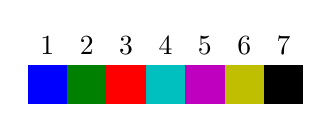
\begin{tikzpicture}[scale=0.5]
        \foreach \x/\c in {1/bb, 2/gg, 3/rr, 4/cc, 5/mm, 6/yy, 7/kk} {
            \fill[\c] (\x, 0) rectangle ++(1,1);
            \path (\x,1) ++ (right:0.5) node[above] {\x};
        };
    \end{tikzpicture}
    \caption{Color order for sweep plots in the report.}
    \label{fig:colororder}
\end{figure}

When two-port S-parameter measurements are mentioned in the report, port 1 is always the top-antenna and port 2 is the side-antenna unless otherwise noted.

